\documentclass[11pt, oneside]{article}   	% use "amsart" instead of "article" for AMSLaTeX format
\usepackage{geometry}                		% See geometry.pdf to learn the layout options. There are lots.
\geometry{letterpaper}                   		% ... or a4paper or a5paper or ... 
%\geometry{landscape}                		% Activate for for rotated page geometry
%\usepackage[parfill]{parskip}    		% Activate to begin paragraphs with an empty line rather than an indent
\usepackage{graphicx}								% TeX will automatically convert eps --> pdf in pdflatex		
\usepackage{amsmath, amsthm, amssymb, bbm,stmaryrd}
\usepackage{hyperref}
\usepackage[round]{natbib}
\usepackage{color}
\usepackage{array}
\usepackage{float}
\usepackage{url}
\usepackage{wrapfig}
\usepackage{listings}
% for proper bold math, including bold greek letters; typesets in math-mode
% and not in \mathrm font
\usepackage{bm}

\usepackage{amsopn}

% \va, \vb etc. type bold letters; notice exception at \vech -- coz. \vh is a
% predefined thing in latex; 
% additional commands include \vah -- read as vector a hat, 
% or \ah -- a hat and so on
\newcommand{\va}{\bm{a}}       \newcommand{\vah}{\hat{\bm{a}}}        \newcommand{\ah}{\hat{a}}
\newcommand{\vb}{\bm{b}}       \newcommand{\vbh}{\hat{\bm{b}}}        \newcommand{\bh}{\hat{b}}
\newcommand{\vc}{\bm{c}}       \newcommand{\vch}{\hat{\bm{c}}}        \newcommand{\ch}{\hat{c}}
\newcommand{\vd}{\bm{d}}       \newcommand{\vdh}{\hat{\bm{d}}}        \newcommand{\dhat}{\hat{d}}
\newcommand{\ve}{\bm{e}}       \newcommand{\veh}{\hat{\bm{e}}}        \newcommand{\eh}{\hat{e}}
\newcommand{\vf}{\bm{f}}       \newcommand{\vfh}{\hat{\bm{f}}}        \newcommand{\fh}{\hat{f}}
\newcommand{\vg}{\bm{g}}       \newcommand{\vgh}{\hat{\bm{g}}}        \newcommand{\gh}{\hat{g}}
\newcommand{\vech}{\bm{h}}     \newcommand{\vhh}{\hat{\bm{h}}}        \newcommand{\hh}{\hat{h}}
\newcommand{\vi}{\bm{i}}       \newcommand{\vih}{\hat{\bm{i}}}        \newcommand{\ih}{\hat{i}}
\newcommand{\vj}{\bm{j}}       \newcommand{\vjh}{\hat{\bm{j}}}        \newcommand{\jh}{\hat{j}}
\newcommand{\vk}{\bm{k}}       \newcommand{\vkh}{\hat{\bm{k}}}        \newcommand{\kh}{\hat{k}}
\newcommand{\vl}{\bm{l}}       \newcommand{\vlh}{\hat{\bm{l}}}        \newcommand{\lh}{\hat{l}}
\newcommand{\vm}{\bm{m}}       \newcommand{\vmh}{\hat{\bm{m}}}        \newcommand{\mh}{\hat{m}}
\newcommand{\vn}{\bm{n}}       \newcommand{\vnh}{\hat{\bm{n}}}        \newcommand{\nh}{\hat{n}}
\newcommand{\vo}{\bm{o}}       \newcommand{\voh}{\hat{\bm{o}}}        \newcommand{\oh}{\hat{o}}
\newcommand{\vp}{\bm{p}}       \newcommand{\vph}{\hat{\bm{p}}}        \newcommand{\ph}{\hat{p}}
\newcommand{\vq}{\bm{q}}       \newcommand{\vqh}{\hat{\bm{q}}}        \newcommand{\qh}{\hat{q}}
\newcommand{\vr}{\bm{r}}       \newcommand{\vrh}{\hat{\bm{r}}}        \newcommand{\rh}{\hat{r}}
\newcommand{\vs}{\bm{s}}       \newcommand{\vsh}{\hat{\bm{s}}}        \newcommand{\sh}{\hat{s}}
\newcommand{\vt}{\bm{t}}       \newcommand{\vth}{\hat{\bm{t}}}        \newcommand{\that}{\hat{t}}
\newcommand{\vu}{\bm{u}}       \newcommand{\vuh}{\hat{\bm{u}}}        \newcommand{\uh}{\hat{u}}
\newcommand{\vv}{\bm{v}}       \newcommand{\vvh}{\hat{\bm{v}}}        \newcommand{\vh}{\hat{v}}
\newcommand{\vw}{\bm{w}}       \newcommand{\vwh}{\hat{\bm{w}}}        \newcommand{\wh}{\hat{w}}
\newcommand{\vx}{\bm{x}}       \newcommand{\vxh}{\hat{\bm{x}}}        \newcommand{\xh}{\hat{x}}
\newcommand{\vy}{\bm{y}}       \newcommand{\vyh}{\hat{\bm{y}}}        \newcommand{\yh}{\hat{y}}
\newcommand{\vz}{\bm{z}}       \newcommand{\vzh}{\hat{\bm{z}}}        \newcommand{\zh}{\hat{z}}

% %%%%%%%%%%%%%%%%%%%% BOLD GREEK %%%%%%%%%%%%%%%%%%%%%%%%%%%%% 
% Same convention as for ordinary roman letters above
\newcommand{\valpha}  {\bm{\alpha}}      \newcommand{\valphah}  {\hat{\bm{\alpha}}}   
\newcommand{\vbeta}   {\bm{\beta}}       \newcommand{\vbetah}   {\hat{\bm{\beta}}}    
\newcommand{\vdelta}  {\bm{\delta}}      \newcommand{\vdeltah}  {\hat{\bm{\delta}}}   
\newcommand{\vepsilon}{\bm{\epsilon}}    \newcommand{\vepsilonh}{\hat{\bm{\epsilon}}} 
\newcommand{\vphi}    {\bm{\phi}}        \newcommand{\vphih}    {\hat{\bm{\phi}}}     
\newcommand{\vgamma}  {\bm{\gamma}}      \newcommand{\vgammah}  {\hat{\bm{\gamma}}}   
\newcommand{\veta}    {\bm{\eta}}        \newcommand{\vetah}    {\hat{\bm{\eta}}}     
\newcommand{\vtheta}  {\bm{\theta}}      \newcommand{\vthetah}  {\hat{\bm{\theta}}}   
\newcommand{\vkappa}  {\bm{\kappa}}      \newcommand{\vkappah}  {\hat{\bm{\kappa}}}   
\newcommand{\vlambda} {\bm{\lambda}}     \newcommand{\vlambdah} {\hat{\bm{\lambda}}}  
\newcommand{\vmu}     {\bm{\mu}}         \newcommand{\vmuh}     {\hat{\bm{\mu}}}      
\newcommand{\vnu}     {\bm{\nu}}         \newcommand{\vnuh}     {\hat{\bm{\nu}}}      
\newcommand{\vpi}     {\bm{\pi}}         \newcommand{\vpih}     {\hat{\bm{\pi}}}      
\newcommand{\vchi}    {\bm{\chi}}        \newcommand{\vchih}    {\hat{\bm{\chi}}}     
\newcommand{\vrho}    {\bm{\rho}}        \newcommand{\vrhoh}    {\hat{\bm{\rho}}}     
\newcommand{\vsigma}  {\bm{\sigma}}      \newcommand{\vsigmah}  {\hat{\bm{\sigma}}}   
\newcommand{\vtau}    {\bm{\tau}}        \newcommand{\vtauh}    {\hat{\bm{\tau}}}     
\newcommand{\vupsilon}{\bm{\upsilon}}    \newcommand{\vupsilonh}{\hat{\bm{\upsilon}}} 
\newcommand{\vomega}  {\bm{\omega}}      \newcommand{\vomegah}  {\hat{\bm{\omega}}}   
\newcommand{\vxi}     {\bm{\xi}}         \newcommand{\vxih}     {\hat{\bm{\xi}}}      
\newcommand{\vpsi}    {\bm{\psi}}        \newcommand{\vpsih}    {\hat{\bm{\psi}}}     
\newcommand{\vzeta}   {\bm{\zeta}}       \newcommand{\vzetah}   {\hat{\bm{\zeta}}}

% %%%%%%%%%%%%%  MATRICES %%%%%%%%%%%%%%%%%%%%%%%%%%%%%  
\newcommand{\ma}{\bm{A}}       \newcommand{\mah}{\hat{\bm{A}}}   
\newcommand{\mb}{\bm{B}}       \newcommand{\mbh}{\hat{\bm{B}}}   
\newcommand{\mc}{\bm{C}}       \newcommand{\mch}{\hat{\bm{C}}}   
\newcommand{\md}{\bm{D}}       \newcommand{\mdh}{\hat{\bm{D}}}   
\newcommand{\me}{\bm{E}}       \newcommand{\meh}{\hat{\bm{E}}}   
\newcommand{\mf}{\bm{F}}       \newcommand{\mfh}{\hat{\bm{F}}}   
\newcommand{\mg}{\bm{G}}       \newcommand{\mgh}{\hat{\bm{G}}}   
\newcommand{\mH}{\bm{H}}       \newcommand{\mhh}{\hat{\bm{H}}}   
\newcommand{\mi}{\bm{I}}       \newcommand{\mih}{\hat{\bm{I}}}   
\newcommand{\mj}{\bm{J}}       \newcommand{\mjh}{\hat{\bm{J}}}   
\newcommand{\mk}{\bm{K}}       \newcommand{\mkh}{\hat{\bm{K}}}   
\newcommand{\ml}{\bm{L}}       \newcommand{\mlh}{\hat{\bm{L}}}   
\newcommand{\mm}{\bm{M}}       \newcommand{\mmh}{\hat{\bm{M}}}   
\newcommand{\mn}{\bm{N}}       \newcommand{\mnh}{\hat{\bm{N}}}   
\newcommand{\mo}{\bm{O}}       \newcommand{\moh}{\hat{\bm{O}}}   
\newcommand{\mP}{\bm{P}}       \newcommand{\mph}{\hat{\bm{P}}}   
\newcommand{\mq}{\bm{Q}}       \newcommand{\mqh}{\hat{\bm{Q}}}   
\newcommand{\mr}{\bm{R}}       \newcommand{\mrh}{\hat{\bm{R}}}   
\newcommand{\ms}{\bm{S}}       \newcommand{\msh}{\hat{\bm{S}}}   
\newcommand{\mT}{\bm{T}}       \newcommand{\mth}{\hat{\bm{T}}}   
\newcommand{\mU}{\bm{U}}       \newcommand{\muh}{\hat{\bm{U}}}   
\newcommand{\mv}{\bm{V}}       \newcommand{\mvh}{\hat{\bm{V}}}   
\newcommand{\mw}{\bm{W}}       \newcommand{\mwh}{\hat{\bm{W}}}   
\newcommand{\mx}{\bm{X}}       \newcommand{\mxh}{\hat{\bm{X}}}   
\newcommand{\my}{\bm{Y}}       \newcommand{\myh}{\hat{\bm{Y}}}   
\newcommand{\mz}{\bm{Z}}       \newcommand{\mzh}{\hat{\bm{Z}}}   

%%%%%%%%%%%%%%%%%%%%%%%%% CALLIGRAPHIC LETTERS %%%%%%%%%%%%%%%%%%%%%
\newcommand{\ac}{\mathcal{a}}    \newcommand{\Ac}{\mathcal{A}}  
\newcommand{\bc}{\mathcal{b}}    \newcommand{\Bc}{\mathcal{B}}  
\newcommand{\cc}{\mathcal{c}}    \newcommand{\Cc}{\mathcal{C}}  
\newcommand{\dc}{\mathcal{d}}    \newcommand{\Dc}{\mathcal{D}}  
\newcommand{\ec}{\mathcal{e}}    \newcommand{\Ec}{\mathcal{E}}  
\newcommand{\fc}{\mathcal{f}}    \newcommand{\Fc}{\mathcal{F}}  
\newcommand{\gc}{\mathcal{g}}    \newcommand{\Gc}{\mathcal{G}}  
\newcommand{\hc}{\mathcal{h}}    \newcommand{\Hc}{\mathcal{H}}  
\newcommand{\ic}{\mathcal{i}}    \newcommand{\Ic}{\mathcal{I}}  
\newcommand{\jc}{\mathcal{j}}    \newcommand{\Jc}{\mathcal{J}}  
\newcommand{\kc}{\mathcal{k}}    \newcommand{\Kc}{\mathcal{K}}  
\newcommand{\lc}{\mathcal{l}}    \newcommand{\Lc}{\mathcal{L}}  
\newcommand{\mcal}{\mathcal{m}}  \newcommand{\Mc}{\mathcal{M}}  
\newcommand{\nc}{\mathcal{n}}    \newcommand{\Nc}{\mathcal{N}}  
\newcommand{\oc}{\mathcal{o}}    \newcommand{\Oc}{\mathcal{O}}  
\newcommand{\pc}{\mathcal{p}}    \newcommand{\Pc}{\mathcal{P}}  
\newcommand{\qc}{\mathcal{q}}    \newcommand{\Qc}{\mathcal{Q}}  
\newcommand{\rc}{\mathcal{r}}    \newcommand{\Rc}{\mathcal{R}}  
\newcommand{\scal}{\mathcal{s}}  \newcommand{\Sc}{\mathcal{S}}  
\newcommand{\tc}{\mathcal{t}}    \newcommand{\Tc}{\mathcal{T}}  
\newcommand{\uc}{\mathcal{u}}    \newcommand{\Uc}{\mathcal{U}}  
\newcommand{\vcal}{\mathcal{v}}  \newcommand{\Vc}{\mathcal{V}}  
\newcommand{\wc}{\mathcal{w}}    \newcommand{\Wc}{\mathcal{W}}  
\newcommand{\xc}{\mathcal{x}}    \newcommand{\Xc}{\mathcal{X}}  
\newcommand{\yc}{\mathcal{y}}    \newcommand{\Yc}{\mathcal{Y}}  
\newcommand{\zc}{\mathcal{z}}    \newcommand{\Zc}{\mathcal{Z}}  

% ================= NORMS ===========================
\newcommand{\mynorm}[2]{\| {#1} \|_{#2}}
\newcommand{\norm}[2]{\mynorm{#1}{#2}}

\newcommand{\onenorm}[1]{\mynorm{#1}{1}}
\newcommand{\bigonenorm}[1]{\bignorm{#1}{1}}

\newcommand{\infnorm}[1]{\mynorm{#1}{\infty}}
\newcommand{\biginfnorm}[1]{\bignorm{#1}{\infty}}

\newcommand{\oneinf}{\ell_{1,\infty}}
\newcommand{\onetwo}{\ell_{1,2}}
\newcommand{\oneinfnorm}[1]{\mynorm{#1}{1,\infty}}
\newcommand{\bigoneinfnorm}[1]{\bignorm{#1}{1,\infty}}

\newcommand{\onetwonorm}[1]{\mynorm{#1}{1,2}}
\newcommand{\bigonetwonorm}[1]{\bignorm{#1}{1,2}}

\newcommand{\twonorm}[1]{\mynorm{#1}{2}}
\newcommand{\bigtwonorm}[1]{\bignorm{#1}{2}}

\newcommand{\znorm}[1]{\mynorm{#1}{0}}
\newcommand{\bigznorm}[1]{\bignorm{#1}{0}}

\newcommand{\frob}[1]{\|{#1}\|_{\text{F}}}
\newcommand{\bigfrob}[1]{\bignorm{#1}{\text{F}}}


% ================ SUMs, INTEGRALS, WITHOUT LIMITS ================
\newcommand{\nlsum}{\sum\nolimits}
\newcommand{\nlprod}{\prod\nolimits}
\newcommand{\nlint}{\int\nolimits}
\newcommand{\nlmin}{\min\nolimits}
\newcommand{\indicator}[1]{\mathbbm{1}\!\left[#1\right]}

% =============== USEFUL SETS, FIELDS, ETC. ===========================
\newcommand{\R}{\mathbb{R}}
\newcommand{\N}{\mathbb{N}}
\newcommand{\reals}{\mathbb{R}}
\newcommand{\complex}{\matbb{C}}
\newcommand{\integers}{\mathbb{Z}}
\newcommand{\posdef}[1]{S_{++}^{#1}}
\newcommand{\semidef}[1]{S_+^{#1}}

% =============== MISC CONSTANTS ============================
\newcommand{\half}{\tfrac{1}{2}}
\newcommand{\third}{\tfrac{1}{3}}
\newcommand{\fourth}{\tfrac{1}{4}}
\newcommand{\onehalf}{\tfrac{3}{2}}

% %%%%%%%%%%% MATH KEYWORDS %%%%%%%%%%%%%%%%%%%%%%%%%%
\DeclareMathOperator*{\argmin}{argmin}
\DeclareMathOperator*{\argmax}{argmax}
\DeclareMathOperator{\dom}{dom}
\DeclareMathOperator{\interior}{int}
\DeclareMathOperator{\rank}{rank}
\DeclareMathOperator{\ri}{ri}
\DeclareMathOperator{\sgn}{sgn}
\DeclareMathOperator{\trace}{Tr}
\DeclareMathOperator{\Diag}{Diag}
\DeclareMathOperator{\range}{range}
\DeclareMathOperator{\vect}{vec}
\DeclareMathOperator{\prox}{prox}
\DeclareMathOperator{\intr}{int}
\DeclareMathOperator{\relint}{ri}

% === References to figures, theorems, etc. ===
\newcommand{\prop}[1]{Proposition~\protect\ref{#1}}
\newcommand{\coro}[1]{Corollary~\protect\ref{#1}}
\newcommand{\rema}[1]{Remark~\protect\ref{#1}}
\newcommand{\exam}[1]{Example~\protect\ref{#1}}
\newcommand{\appl}[1]{Application~\protect\ref{#1}}
% [SN]: lowercase \algo, uppercase \Algo
\newcommand{\Algo}[1]{Algorithm~\protect\ref{#1}}
\newcommand{\algo}[1]{Algorithm~\protect\ref{#1}}
\newcommand{\opti}[1]{Optimization Problem~\protect\ref{#1}}
\newcommand{\defi}[1]{Definition~\protect\ref{#1}}
\newcommand{\prob}[1]{Problem~\protect\ref{#1}}
% [SN]: lowercase \theo, uppercase \Theo
\newcommand{\Theo}[1]{Theorem~\protect\ref{#1}}
\newcommand{\theo}[1]{Theorem~\protect\ref{#1}}
% [SN]: lowercase \fig, uppcase \Fig
\newcommand{\Fig}[1]{Figure~\protect\ref{#1}}
\newcommand{\fig}[1]{Figure~\protect\ref{#1}}
\newcommand{\tab}[1]{Table~\protect\ref{#1}}
\newcommand{\chap}[1]{Chapter~\protect\ref{#1}}
% [SN]: lowercase \sec, uppcase \Sec
% TODO: check all occurences of \sec at the beginning of a sentence
\newcommand{\Sec}[1]{Section~\protect\ref{#1}}
\renewcommand{\sec}[1]{Section~\protect\ref{#1}} % SS: but why?????? it shd always be uppercase!
\newcommand{\app}[1]{Appendix~\protect\ref{#1}}
\newcommand{\eq}[1]{(\protect\ref{#1})}
\newcommand{\pag}[1]{page \protect\pageref{#1}}

% === Marginal notes ===
% To use marginal notes, type in \margin{this goes into the margin}
\newcommand{\margin}[1]{\marginpar[\flushleft{#1}]{right}}


%%% our settings %%%
\newcommand{\expectation}{\mathbb{E}}
\newcommand{\ex}[1]{e^{#1}}
\newcommand{\stred}{\textsc{StructED}~}
\newcommand{\comment}[1]{\noindent{\textcolor{red}{#1}}}

\usepackage{color}

\definecolor{dkgreen}{rgb}{0,0.6,0}
\definecolor{gray}{rgb}{0.5,0.5,0.5}
\definecolor{mauve}{rgb}{0.58,0,0.82}

\lstset{frame=tb,
  language=Java,
  aboveskip=3mm,
  belowskip=3mm,
  showstringspaces=false,
  columns=flexible,
  basicstyle={\small\ttfamily},
  numbers=none,
  numberstyle=\tiny\color{gray},
  keywordstyle=\color{blue},
  commentstyle=\color{dkgreen},
  stringstyle=\color{mauve},
  breaklines=true,
  breakatwhitespace=true,
  tabsize=3
}

\sloppy
\title{\centerline{
\includegraphics[width=7cm]{img/logo.png}}}
\author{Tutorial - \href{http://adiyoss.github.io/}{by Adiyoss}}
%\date{}		% Activate to display a given date or no date

\begin{document}
\maketitle
\section{Introduction}
In this tutorial we will demonstrate how to use and add new task to the \stred package. We will give code examples for the Task-Loss, Predict - Inference and Feature Functions interfaces, as well as update for the Factory class. For this tutorial we will use small subset from a dummy data that was generated in our lab in order to debug the vowel duration measurement problem, where the input is a speech segment and the output is the onset and offset of the vowel, meaning the start time and end time of the vowel.
\section{Dummy Data}
The dummy data we use in this tutorial was generated in order to debug the vowel duration measurement problem. Hence, the label for each example is composed from two numbers, the start time and end time ($Y\in{\mathbb{R}}^2$), and the input data is an arbitrary length vector of numbers for 0,1 domain, ($X \in{\{0,1\}}^d$ and $d\in{\mathbb{N}}$). \\
For example: 

8-17 0:0 1:0 2:1 3:0 4:0 5:0 6:0 7:0 8:1 9:1 10:1 11:0 12:1 13:1 14:1 15:1 16:1 17:0 18:0 19:0\\
Here, the first two numbers are the label which indicates that the signal turns on at the eighth element of the vector and turns off at the seventeenth element of the vector. Each vector data is composed from the index of the feature, we did this to support space features, and the feature data separated by a colon(:). Our goal is to find a function $\emph{f}$ that gets as input the vector data and outputs the start time where the signal turns on and end time where it turns off. Notice, we add a little bit off noise to the vector data for example at the second index or at the eleventh index, we want to fine $\emph{f}$ that isn't sensitive to small amount of noise in the data. We know that this is a toy example, but it demonstrate really good the use of the package and the integration with it. We assume that the signal turns on only once.

The db can be found under the db/dummy folder in the project repository.

\section{The Code}
Here, we present        lasses do we need to add and what interfaces do we need to implement. We provide the source code for each class and interface.
\subsection{Task Loss}
We now add a task loss class. Every task loss class should implement the TaskLoss interface. In our problem settings we use the following task loss: 

\begin{equation}
\label{eq:loss}
\ell ((t_{s}, t_{e}),(\hat{t_{s}}, \hat{t_{e}})) = max{\{|(\hat{t_{s}}-\hat{t_{e}}) - (t_{s} - t_{e})| - \epsilon ,0\}}
\end{equation} 
In words, the loss will be the max between zero to the difference between the predicted signals length to its actual length and we minus epsilon. This means that we allow the classifier to be mistaken by at most epsilon.

For this we create new java class inside the TaskLoss package, this class should implement the TaskLoss interface, we put the following code in it:
\begin{lstlisting}
package BL.TaskLoss;

import Constants.Consts;
import java.util.List;

public class TaskLossDummyData implements TaskLoss {

	@Override
	//max{0,|ys-ye - y's-y'e|-epsilon}
	public double computeTaskLoss(String predictClass, String actualClass, List<Double> params) {
        double epsilon = params.get(0);
		String predictValues[] = predictClass.split(Consts.CLASSIFICATION_SPLITTER);
		String actualClassValues[] = actualClass.split(Consts.CLASSIFICATION_SPLITTER);
	
		//calculate difference of each classification
		double predictRes = Double.parseDouble(predictValues[0]) - Double.parseDouble(predictValues[1]);
		double actualRes = Double.parseDouble(actualClassValues[0]) - Double.parseDouble(actualClassValues[1]);
		
		//subtract the epsilon		
		double absRes = Math.abs(predictRes-actualRes) - epsilon;
		
		//get the max from the absolute result minus epsilon and 0
		if(absRes > 0)
			return absRes;
		return 0;
	}
}
\end{lstlisting}

\subsection{Predict - Inference}
We now add a predict/inference class. Every predict class should implement the Prediction interface. In our problem settings the prediction will be brute force. To make the code go faster we assume that at the beginning and end there's a gap of three frames, which means the beginning of the of the signal can't be in the first 3 frames and the end of the signal can't be at the last three frames, this can be defined other wise if needed. We go over all the possible time sequences for the start time start from minimum gap to maximum gap. Inside an inner loop we go from the start location to minimum gap at the end. The inner loop can also be optimize by start from the minimum length possible of the signal to the maximum length possible of the signal.

In general we need the prediction class to implement the following:

\begin{equation}
\label{eq:decoding}
\vyh_{\vw}(\vx) = \argmax_{\vy \in \Yc} ~ \vw^\top \vphi(\vx, \vy)
\end{equation}
and,

\begin{equation}
\label{eq:augmented-loss}
\vyh_{\vw}(\vx) = \argmax_{\vyh \in \Yc} ~ \vw^\top \vphi(\vx, \vyh) + \ell (\vy,\vyh)
\end{equation}

For this we create new java class inside the Prediction package, this class should implement the Prediction interface, we put the following code in it:

\begin{lstlisting}
package BL.Prediction;

import BL.ClassifierData;
import Constants.Consts;
import Constants.ErrorConstants;
import Data.Entities.Example;
import Data.Entities.PredictedLabels;
import Data.Entities.Vector;
import Helpers.Comperators.MapValueComparatorDescending;
import Helpers.MathHelpers;

public class PredictionDummyData implements Prediction {

    //predict function
    //argmax(yS,yE) (W*Phi(Xi,yS,yE)) + Task Loss
    //this function assumes that the argument vector has already been converted to phi vector
    //return null on error
    public PredictedLabels predictForTrain(Example vector, Vector W, String realClass, ClassifierData classifierData, double epsilon, double epsilonArgMax)
    {
        try{
            PredictedLabels tree = new PredictedLabels();

            //validation
            if(vector.sizeOfVector<=0)
            {
                System.err.println(ErrorConstants.PHI_VECTOR_DATA);
                return null;
            }

            //loop over all the classifications of this specific example
            for(int i=Consts.MIN_GAP_START_DUMMY-1 ; i<vector.sizeOfVector-Consts.MIN_GAP_END_DUMMY ; i++)
            {
                for(int j=i+1 ; j<vector.sizeOfVector- Consts.MIN_GAP_END_DUMMY ; j++)
                {
                    Example phiData = classifierData.phi.convert(vector,(i+1)+ Consts.CLASSIFICATION_SPLITTER+(j+1),classifierData.kernel);
                    //multiple the vectors
                    double tmp = MathHelpers.multipleVectors(W, phiData.getFeatures());

                    if(epsilonArgMax != 0){
                        //add the task loss
                        tmp += epsilonArgMax*classifierData.taskLoss.computeTaskLoss((i+1)+ Consts.CLASSIFICATION_SPLITTER+(j+1), realClass, classifierData.arguments);
                    }

                    //get the max value for the max classification
                    tree.put((i+1)+ Consts.CLASSIFICATION_SPLITTER+(j+1),tmp);
                }
            }

            MapValueComparatorDescending vc = new MapValueComparatorDescending(tree);
            PredictedLabels result = new PredictedLabels(vc);
            result.putAll(tree);

            return result;

        } catch (Exception e){
            e.printStackTrace();
            return null;
        }
    }

    public PredictedLabels predictForTest(Example vector, Vector W, String realClass, ClassifierData classifierData, int returnAll)
    {
        return predictForTrain(vector,W,realClass,classifierData,0,0);
    }
}
\end{lstlisting}

\subsection{Feature Functions}
We now add the feature functions. Every feature function class should implement the PhiConvertor interface. Since we want to recognize the pick of the start of the signal  and the decrease of the end signal we implemented the following feature functions:

\begin{enumerate}
  \item Difference between the element at the start index to the element at index start - 1
  \item Difference between the element at the start index to the element at index start - 2
  \item Difference between the element at the end index to the element at index end + 1
  \item Difference between the element at the end index to the element at index end + 2
  \item Difference between the mean of the signal from start to end to the mean of the signal from start to start - 3
  \item Difference between the mean of the signal from start to end to the mean of the signal from end to end + 3
\end{enumerate}

We expect that the value of the above feature functions will be high when we reach the true start time and end time, and low otherwise.

For this we create new java class inside the FeatureFunction package, this class should implement the PhiConverter interface, we put the following code in it:
\begin{lstlisting}
package Data.FeatureFunctions;

import BL.Kernels.Kernel;
import Constants.Consts;
import Constants.ErrorConstants;
import Data.Entities.Example;
import Data.Entities.Vector;
import Data.Factory;

public class PhiDummyConverter implements PhiConverter {

    int sizeOfVector = 4;

	@Override
	//return null on error
	public Example convert(Example vector, String label, Kernel kernel) {

        try{
            Example newVector = Factory.getExample(0);

            String labelValues[] = label.split(Consts.CLASSIFICATION_SPLITTER);
            int i = Integer.parseInt(labelValues[0]);
            int j = Integer.parseInt(labelValues[1]);

            //compute the difference/gradients near the start and end points
            double diff_1_Start = Math.abs(vector.getFeatures().get(i)-vector.getFeatures().get(i-1));
            double diff_1_End = Math.abs(vector.getFeatures().get(j)-vector.getFeatures().get(j+1));

            //compute the difference/gradients near the start and end points
            double diff_2_Start = Math.abs(vector.getFeatures().get(i)-vector.getFeatures().get(i-2));
            double diff_2_End = Math.abs(vector.getFeatures().get(j)-vector.getFeatures().get(j+2));

	    		//compute the avg of the signal from start to end
            double avg = 0;
            for(int k=i ; k<j ; k++)
                avg+=vector.getFeatures().get(k);

            if(j-i <= 0){
                System.err.println("Convert single vector: "+ ErrorConstants.GENERAL_ERROR+ ErrorConstants.ZERO_DIVIDING);
                return null;
            }
            avg /= (double)(j-i);


				//compute the avg MIN_GAP_END_DUMMY  after end
            double gapEnd = 0;
            for(int k=j ; k<j+Consts.MIN_GAP_END_DUMMY ; k++)
                gapEnd+=vector.getFeatures().get(k);

            gapEnd/=(double)Consts.MIN_GAP_END_DUMMY;
				//compute the avg MIN_GAP_START_DUMMY before start
            double gapStart = 0;
            for(int k=i-Consts.MIN_GAP_START_DUMMY+1 ; k<=i ; k++)
                gapStart+=vector.getFeatures().get(k);

            gapStart/=(double)Consts.MIN_GAP_START_DUMMY;

				//adding the feature functions
            Vector tmpVector = new Vector();
            tmpVector.put(0, diff_1_Start);
            tmpVector.put(1, diff_1_End);
            tmpVector.put(2, diff_2_Start);
            tmpVector.put(3, diff_2_End);
            tmpVector.put(4, avg-gapStart);
            tmpVector.put(5,avg-gapEnd);

            if(kernel!=null)
                tmpVector = kernel.convertVector(tmpVector, sizeOfVector);

            newVector.setFeatures(tmpVector);

            return newVector;

        } catch (Exception e){
            e.printStackTrace();
            return null;
        }
	}
}
\end{lstlisting}

\subsection{Factory Update}
The last code segment we need to add is the update of the Factory class. The factory class is responsible on the creation of all the objects in our package. It gives us the flexibility to add new classes to a new problem that we wish to learn.
We need to add the option to create those new classes that we just implemented. \\ \\ \\
We need to update the getClassifier function to support the creation of those classes, which means just add new case to the relevant switch case statement,  it should look like this: 
\begin{lstlisting}
public static Classifier getClassifier(int taskLossType, int updateType, int predictType, int kernelType, int phi, ArrayList<Double> arguments){
		
		Classifier classifier = new Classifier();
        classifier.classifierData = new ClassifierData();
        classifier.classifierData.arguments = new ArrayList<Double>();
		
		switch (taskLossType) {
			case 0:
                classifier.classifierData.taskLoss = new TaskLossVowelDuration();
				break;
			case 1:
                classifier.classifierData.taskLoss = new TaskLossMultiClass();
				break;
            case 2:
                classifier.classifierData.taskLoss = new TaskLossRank();
                break;
            case 3:
                classifier.classifierData.taskLoss = new TaskLossDummyData();
                break;
			default:
				return null;
		}

        switch (predictType) {
            case 0:
                classifier.classifierData.predict = new PredictionVowelDurationData();
                break;
            case 1:
                classifier.classifierData.predict = new PredictionMultiClass();
                break;
            case 2:
                classifier.classifierData.predict = new PredictionRanking();
                break;
            case 3:
                classifier.classifierData.predict = new PredictionDummyData();
                break;
            default:
                return null;
        }

        switch (phi) {
            case 0:
                classifier.classifierData.phi = new PhiVowelDurationConverter();
                break;
            case 1:
                classifier.classifierData.phi = new PhiSparseConverter();
                break;
            case 2:
                classifier.classifierData.phi = new PhiRankConverter();
                break;
            case 3:
                classifier.classifierData.phi = new PhiDummyConverter();
                break;
            default:
                return null;
        }

        switch (kernelType) {
            case 0:
                classifier.classifierData.kernel = new Poly2Kernel();
                break;
            case 1:
                classifier.classifierData.kernel = new RBF2Kernel();
                break;
            case 2:
                classifier.classifierData.kernel = new RBF3Kernel();
                break;
            default:
                classifier.classifierData.kernel = null;
        }
		
		switch (updateType) {
			case 0:
                classifier.classifierData.algorithmUpdateRule = PassiveAggressive.getInstance(arguments);
				break;
			case 1:
                classifier.classifierData.algorithmUpdateRule = SVM_Pegasos.getInstance(arguments);
				break;
			case 2:
                classifier.classifierData.algorithmUpdateRule = DirectLoss.getInstance(arguments);
				break;
			case 3:
                classifier.classifierData.algorithmUpdateRule = CRF.getInstance(arguments);
				break;
			case 4:
                classifier.classifierData.algorithmUpdateRule = RampLoss.getInstance(arguments);
				break;
			case 5:
                classifier.classifierData.algorithmUpdateRule = ProbitLoss.getInstance(arguments);
				break;
            case 6:
                classifier.classifierData.algorithmUpdateRule = RankSVM.getInstance(arguments);
                break;
			default:
				classifier.classifierData.algorithmUpdateRule = null;
		}

		return classifier;
	}
\end{lstlisting}

We can see here that if we wish to add new Kernel function or even new algorithm, it can be done in the same way.
\section{The Config File}
The last thing we have left to do is update the config file to indicate that we wish to create this classes.
Very detailed information about the Config file can be found at: \href{http://adiyoss.github.io/StructED/}{http://adiyoss.github.io/StructED/} or at the config\_details.txt file which is placed inside the docs folder as well.\\
The config file for the train should look like this(Here we use the Direct-Loss minimization algorithm): \\ \\
train\_path:data/db/dummy/train.txt \\ 
w\_output:data/weights/dummy.weights\\
train\_path:data/db/dummy/train.txt\\
w\_output:data/weights/dummy.weights\\
type:2\\
task:3\\
epoch:5\\
task\_param:1\\
phi:3\\
prediction:3\\
reader:0\\
writer:0\\
size\_of\_vector:4\\
eta:0.5\\
epsilon:-1.6\\
The config file for the prediction should look like this: \\ \\
test\_path:data/db/dummy/test.txt \\
output\_file:res/dummy\_scores.txt \\
w\_path:data/weights/dummy.weights\\
examples\_2\_display:3\\
task:3\\
task\_param:1\\
phi:3\\
prediction:3\\
reader:0\\
writer:0\\
size\_of\_vector:4\\

\section{Running The Code}
To run the code after adding this new classes we need to compile the code for the train and also for the prediction. We can do this either with the IDE that we are working with or from the command line using javac.
Notice, both the train and predict executables requirers the path to the config file as parameter.

The output after the train should look like this: \\ 
\centerline{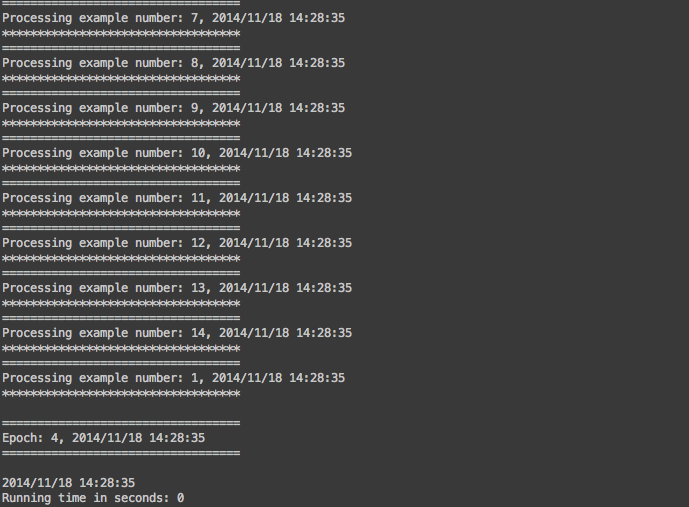
\includegraphics[width=10cm]{img/train.png}}

The output after the prediction should look like this:\\ \\
\centerline{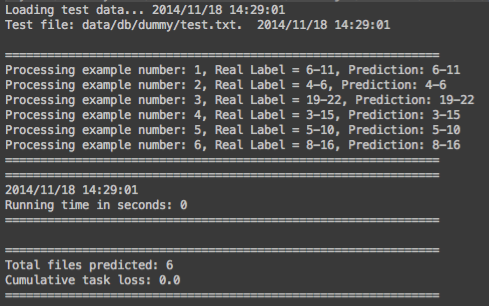
\includegraphics[width=10cm]{img/predict.png}} \\ \\ \\ \\ \\
Hope you had fun!\\
GOOD LUCK! 

\end{document}

